\documentclass[12pt,a4paper]{article}
\newcommand{\AuthorName}
{نام و نام خانوادگی}
\newcommand{\AuthorSTID}
{شماره دانشجویی}

\usepackage{commons/course}
\usetikzlibrary{automata,positioning,arrows.meta}
\tikzset{
->,
>={Stealth[round]},
shorten >=1pt,
thick,
node distance=3cm,
every state/.style={thick, fill=gray!10},
initial text={$ $},
}

\lstset{
numbers=left, 
numberstyle=\small, 
numbersep=8pt, 
frame = single, 
language=Python,
framexleftmargin=15pt
}


%
%\let\ds\displaystyle
%\usepackage{arabtex}
%\usepackage[utf8]{inputenc}
%\usepackage[LFE,LAE]{fontenc}
%\usepackage[english,farsi]{babel}
%


\begin{document}



\سربرگ{تمرین سری اول}{اسکنر و گراف نحو}{99/7/22}



%نام و نام خانوادگی:پارسا نوری
%شماره دانشجویی: ۹۸۲۴۲۳۰۶۷


\مسئله{نام سؤال}

\پاسخ{}

الف)

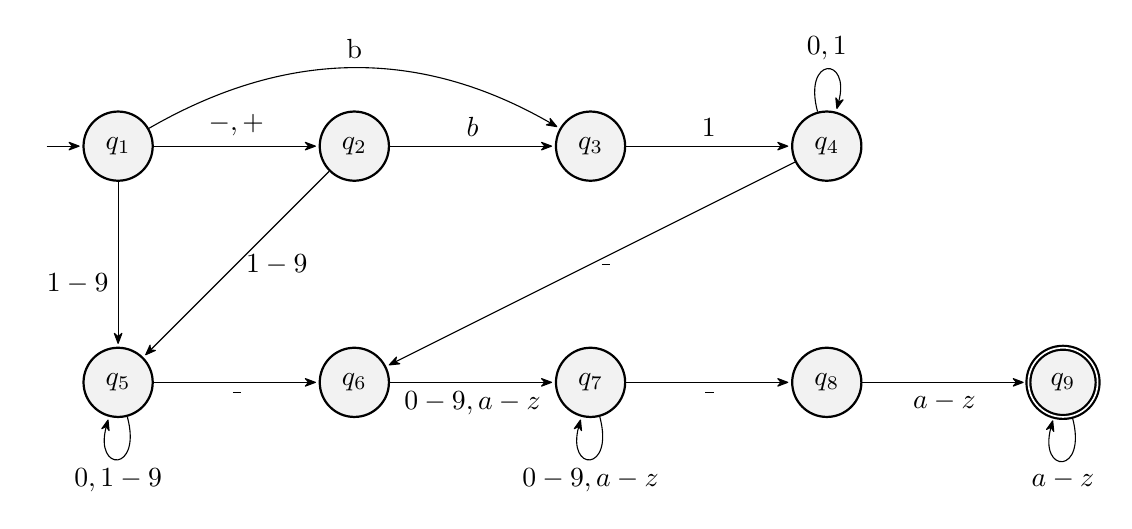
\begin{tikzpicture}
    \node[state,initial] (q1) {$q_1$};
    \node[state] (q2) [right of=q1] {$q_2$};
    \node[state] (q3) [right of=q2]{$q_3$};
    \node[state] (q4) [right of=q3]{$q_4$};
    \node[state] (q5) [below of=q1]{$q_5$};
    \node[state] (q6) [right of=q5]{$q_6$};
    \node[state] (q7) [right of=q6]{$q_7$};
    \node[state] (q8) [right of=q7]{$q_8$};
    \node[state,accepting] (q9) [right of=q8]{$q_9$};
    \draw (q1) edge[above] node{$-,+$} (q2);
    \draw (q1) edge[above] node[below left]{$1-9$} (q5);
    \draw (q1) edge[bend left, above] node{b} (q3);
    \draw (q2) edge[above] node{$b$} (q3);
    \draw (q2) edge[above] node[right]{$1-9$} (q5);
    \draw (q3) edge[above] node{$1$} (q4);
    \draw (q4) edge[loop above] node{$0,1$} (q4);
    \draw (q5) edge[loop below] node{$0,1-9$} (q5);
    %bakhsh e 1 ta inja too q4 o q5 e 
    \draw (q5) edge[above] node[below]{$\_$} (q6);
    \draw (q4) edge[above] node[right]{$\_$} (q6);
    %shoroo e bakhsh e 2
    \draw (q6) edge[above] node[below]{$0-9,a-z$} (q7);
    \draw (q7) edge[loop below] node[below]{$0-9,a-z$} (q7);
    %bakhsh e 2 alan too q7 ok shode
    \draw (q7) edge[above] node[below]{$\_$} (q8);
    \draw (q8) edge[above] node[below]{$a-z$} (q9);
    \draw (q9) edge[loop below] node[below]{$a-z$} (q9);
\end{tikzpicture}

ب)

\begin{latin}
    $((+|-)|\epsilon)((1-9)(0-9)^*|b1(0|1)^+)\_(a-z|0-9)^*\_(a-z)^+$
\end{latin}


%نام و نام خانوادگی:
%شماره دانشجویی: 
\مسئله{نام سؤال}


\پاسخ{}

\lr{Lexical Analyzer DFA} به صورت زیر است:

۱. اگر تنها \lr{token} های \lr{string} را بخواهیم بپذیریم:

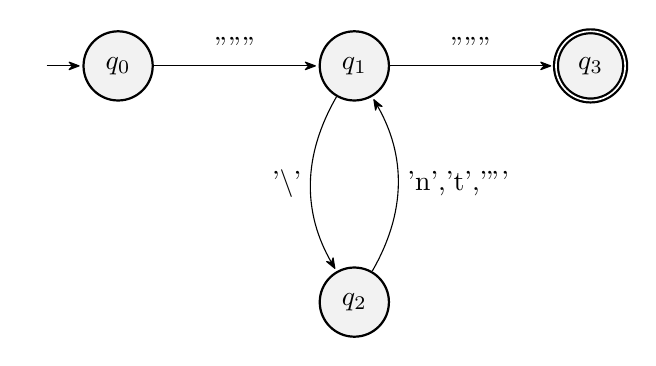
\begin{tikzpicture}

    \node[state,initial] (q0) {$q_0$};
    \node[state,right of=q0] (q1) {$q_1$};
    \node[state,below of=q1] (q2) {$q_2$};
    \node[state,right of=q1,accepting] (q3) {$q_3$};

    \draw (q0) edge[above] node{"""} (q1);
    \draw (q1) edge[bend right] node[left]{'\textbackslash'} (q2);
    \draw (q2) edge[bend right] node[right]{'n','t','"'} (q1);
    \draw (q1) edge[above] node{"""} (q3);

\end{tikzpicture}

۲. اگر قرار باشد که همزمان \lr{token} های \lr{T\_id,T\_str,T\_=} را هم بپذیریم:

در گراف زیر وضعیت \lr{$q_5$} حاکی از \lr{T\_=} و وضعیت \lr{$q_3$} حاکی از \lr{T\_constStr} و \lr{$q_4$} حاکی از \lr{T\_id} میباشند.

\begin{latin}
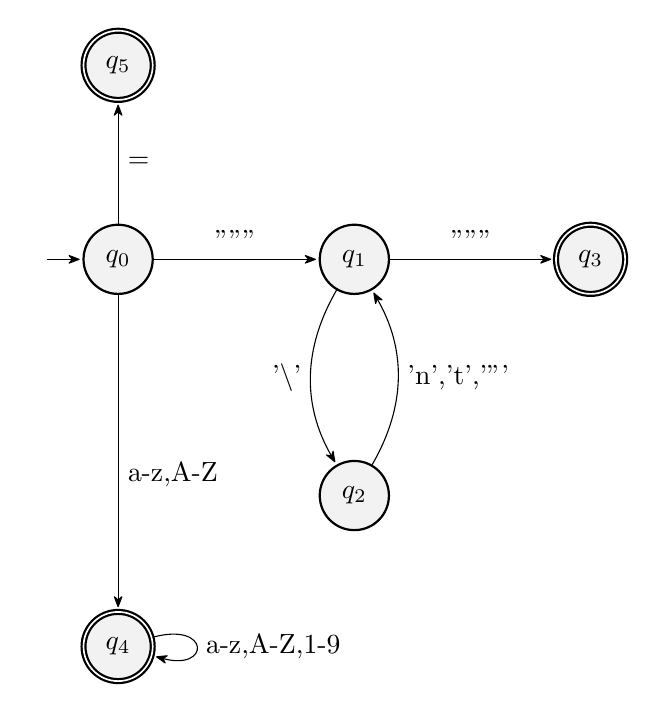
\begin{tikzpicture}

    \node[state,initial] (q0) {$q_0$};
    \node[state,right of=q0] (q1) {$q_1$};
    \node[state,below of=q1] (q2) {$q_2$};
    \node[state,right of=q1,accepting] (q3) {$q_3$};
    \node[state,below=4cm of q0,accepting] (q4) {$q_4$};
    \node[state,above=2cm,accepting] (q5) {$q_5$};

    \draw (q0) edge[above] node{"""} (q1);
    \draw (q1) edge[bend right] node[left]{'\textbackslash'} (q2);
    \draw (q2) edge[bend right] node[right]{'n','t','"'} (q1);
    \draw (q1) edge[above] node{"""} (q3);
    \draw (q0) edge[above] node[below right]{a-z,A-Z} (q4);
    \draw (q4) edge[loop right] node{a-z,A-Z,1-9} (q4);
    \draw (q0) edge[right] node{=} (q5);

\end{tikzpicture}
\end{latin}

کد Scanner به صورت زیر است:

\begin{latin}
    \begin{lstlisting}
#include <iostream>
#include <fstream>
#include <cctype>

using namespace std;

bool is_three_cot(istream &i) {
    auto p = i.tellg();
    bool result = true;
    char c;
    for (int j = 0; j < 3; j++) {
        i.get(c);
        if (c != '"')
            result = false;
    }
    i.seekg(p);
    return result;
}


bool is_id_valid(istream &i) {
    i >> ws;
    char c = i.get();
    if (isdigit(c))
        return false;
    while (i.get(c))
        if (isspace(c))
            return true;
        else if (isalnum(c))
            continue;
        else return false;
    return false;
}

bool is_assigning(istream& i){
    i >> ws;
    return i.get() == '=' ? true : false;

}
bool is_py_str_valid(istream &i) {
    char c;
    i >> ws;
    if (!is_three_cot(i))
        return false;
    i.ignore(3);
    while ((c = i.peek()) != -1) {
        if (is_three_cot(i))
            return true;

        if (c != '\\') {
            i.ignore(1);
            continue;
        }
        i.ignore(1);
        if (is_three_cot(i))
            i.ignore(3);
        else {
            i.ignore(1);
            continue;
        }
    }
    return false;
}
int main() {
    ifstream i("teststr.py");
    if (is_id_valid(i))
        cout << "T_id" << endl;
    if (is_assigning(i))
        cout << "T_=" << endl;
    if (is_py_str_valid(i))
        cout << "T_constStr" << endl;
    return 0;
}
    \end{lstlisting}
\end{latin}


%نام و نام خانوادگی:
%شماره دانشجویی: 
\مسئله{نام سؤال}


\پاسخ{}

%نام و نام خانوادگی:
%شماره دانشجویی: 
\مسئله{نام سؤال}

\پاسخ{}

\begin{latin}
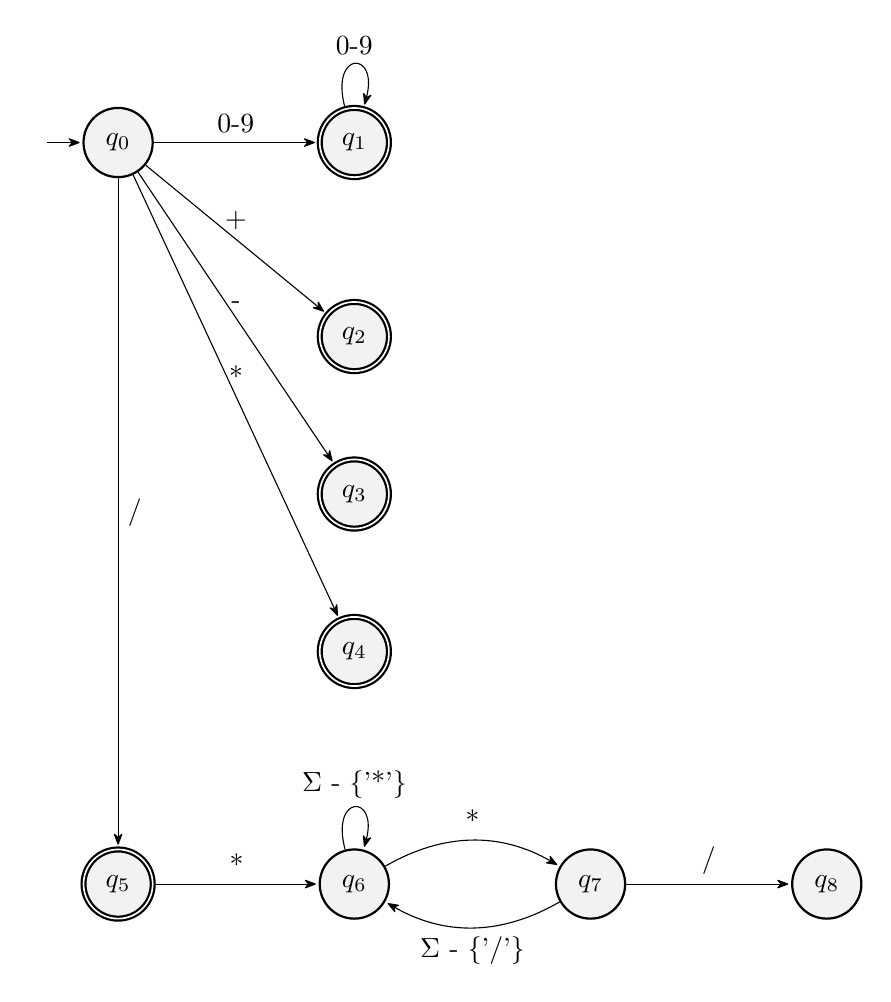
\begin{tikzpicture}
    \node[state, initial] (q0) {$q_0$};
    \node[state,right of=q0,accepting] (q1) {$q_1$};
    \node[state,right of=q0,below=2cm,accepting] (q2) {$q_2$};
    \node[state,right of=q0,below=4cm,accepting] (q3) {$q_3$};
    \node[state,right of=q0,below=6cm,accepting] (q4) {$q_4$};
    \node[state,below=8.5cm of q0,accepting] (q5) {$q_5$};
    \node[state,right of=q5] (q6) {$q_6$};
    \node[state,right of=q6] (q7) {$q_7$};
    \node[state,right of=q7] (q8) {$q_8$};
    
    \draw (q0) edge[above] node{0-9} (q1);
    \draw (q1) edge[loop above] node{0-9} (q1);
    \draw (q0) edge[above] node{+} (q2);
    \draw (q0) edge[above] node{-} (q3);
    \draw (q0) edge[above] node{*} (q4);
    \draw (q0) edge[right] node{/} (q5);
    \draw (q5) edge[above] node{*} (q6);
    \draw (q6) edge[loop above] node{$\Sigma$ - \{'*'\}} (q6);
    \draw (q6) edge[bend left] node[above]{*} (q7);
    \draw (q7) edge[bend left] node[below]{$\Sigma$ - \{'/'\}} (q6);
    \draw (q7) edge[above] node{/} (q8);

\end{tikzpicture}
\end{latin}


%نام و نام خانوادگی:
%شماره دانشجویی: 
\مسئله{نام سؤال}

\پاسخ{}

گراف به صورت زیر است:
در اینجا d بیانگر رقم است.
\begin{latin}
    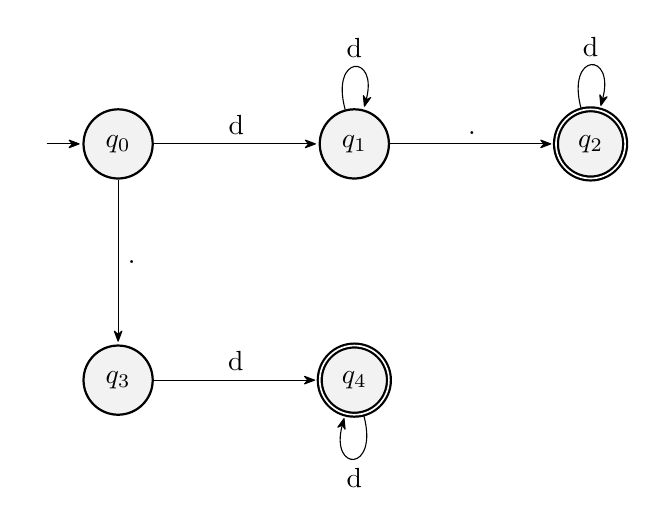
\begin{tikzpicture}
        \node[state,initial] (q0) {$q_0$};
        \node[state,right of=q0] (q1) {$q_1$};
        \node[state,right of=q1,accepting] (q2) {$q_2$};
        \node[state,below of=q0] (q3) {$q_3$};
        \node[state,right of=q3,accepting] (q4) {$q_4$};
        
        \draw (q0) edge[above] node{d} (q1);
        \draw (q1) edge[loop above] node{d} (q1);
        \draw (q1) edge[above] node{.} (q2);
        \draw (q2) edge[loop above] node{d} (q2);
        \draw (q0) edge[right] node{.} (q3);
        \draw (q3) edge[above] node{d} (q4);
        \draw (q4) edge[loop below] node{d} (q4);
    \end{tikzpicture}
\end{latin}
\newpage
کد به صورت زیر است:
\begin{latin}
    \begin{lstlisting}
#include <iostream>
#include <cctype>
using namespace std;

bool is_correct_float(const string& s){
    if (s == ".")
        return false;
    return all_of(s.begin(),s.end(),[] (const char c) -> bool {
        return isdigit(c) || c == '.';
    }) && any_of(s.begin(),s.end(),[] (const char c) -> bool {
        return c == '.';
    });
}
int main()
{
    string s = "2345678.";
    cout << (is_correct_float(s) ? "true" : "false") << endl;
    return 0;
}
    \end{lstlisting}
\end{latin}


%نام و نام خانوادگی:
%شماره دانشجویی: 
\مسئله{نام سؤال}

\پاسخ{}

\begin{latin}
    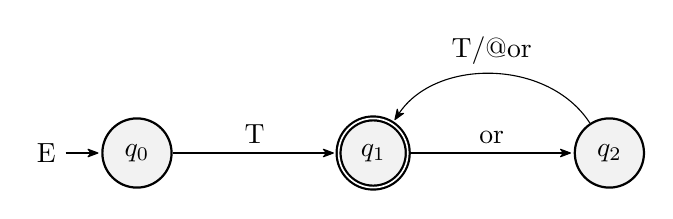
\begin{tikzpicture}
        \node[state,initial,initial text=E] (q0) {$q_0$};
        \node[state,accepting,right of=q0] (q1) {$q_1$};
        \node[state,right of=q1] (q2) {$q_2$};

        \draw (q0) edge[above] node{T} (q1);
        \draw (q1) edge[above] node{or} (q2);
        \draw (q2) edge[bend right=2cm] node[above]{T/@or} (q1);
    \end{tikzpicture}
\end{latin}

\vspace{2cm}

\begin{latin}
    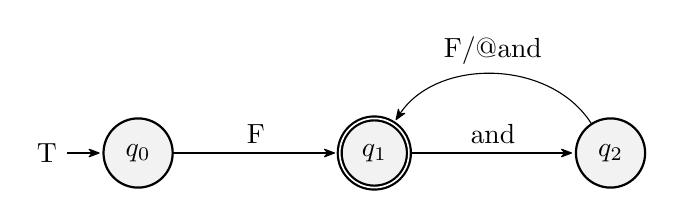
\begin{tikzpicture}
        \node[state,initial,initial text=T] (q0) {$q_0$};
        \node[state,accepting,right of=q0] (q1) {$q_1$};
        \node[state,right of=q1] (q2) {$q_2$};

        \draw (q0) edge[above] node{F} (q1);
        \draw (q1) edge[above] node{and} (q2);
        \draw (q2) edge[bend right=2cm] node[above]{F/@and} (q1);
    \end{tikzpicture}
\end{latin}

\vspace{2cm}

\begin{latin}
    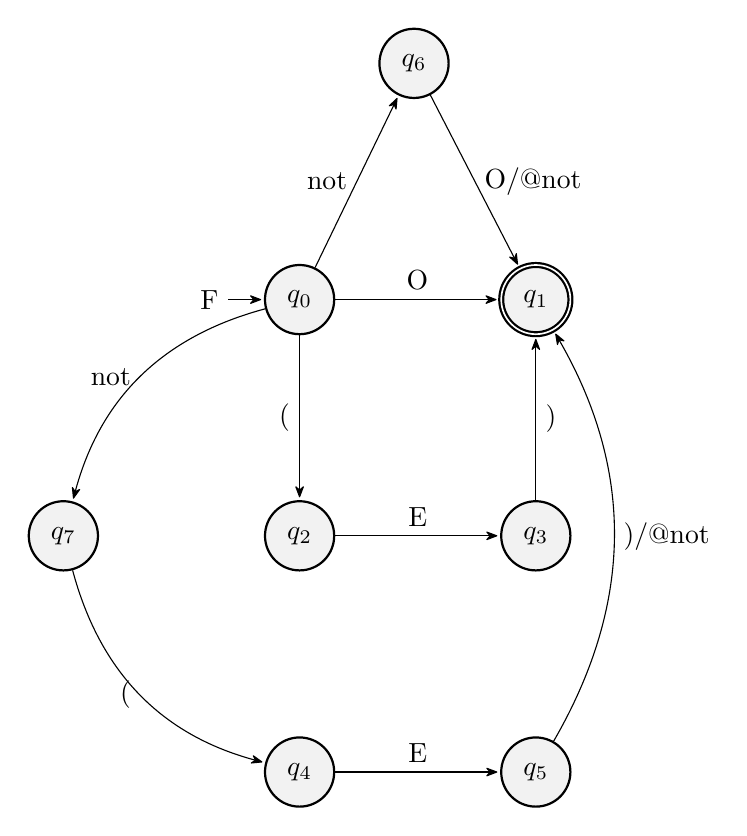
\begin{tikzpicture}
        \node[state,initial,initial text=F] (q0) {$q_0$};
        \node[state,right of=q0,accepting] (q1) {$q_1$};
        \node[state,below of=q0] (q2) {$q_2$};
        \node[state,below of=q1] (q3) {$q_3$};
        \node[state,below of=q2] (q4) {$q_4$};
        \node[state,below of=q3] (q5) {$q_5$};
        \node[state,above of=q0,right=1cm] (q6) {$q_6$};
        \node[state,left of=q2] (q7) {$q_7$};
    
        \draw (q0) edge[above] node{O} (q1);
        \draw (q0) edge[left] node{$($} (q2); 
        \draw (q2) edge[above] node{E} (q3);
        \draw (q3) edge[right] node{$)$} (q1);
        \draw (q0) edge[bend right] node[left]{not} (q7);
        \draw (q7) edge[bend right] node[left]{$($} (q4); 
        \draw (q4) edge[above] node{E} (q5);
        \draw (q5) edge[bend right] node[right]{$)$/@not} (q1);
        \draw (q0) edge[left] node{not} (q6);
        \draw (q6) edge[right] node{O/@not} (q1);
    \end{tikzpicture}

    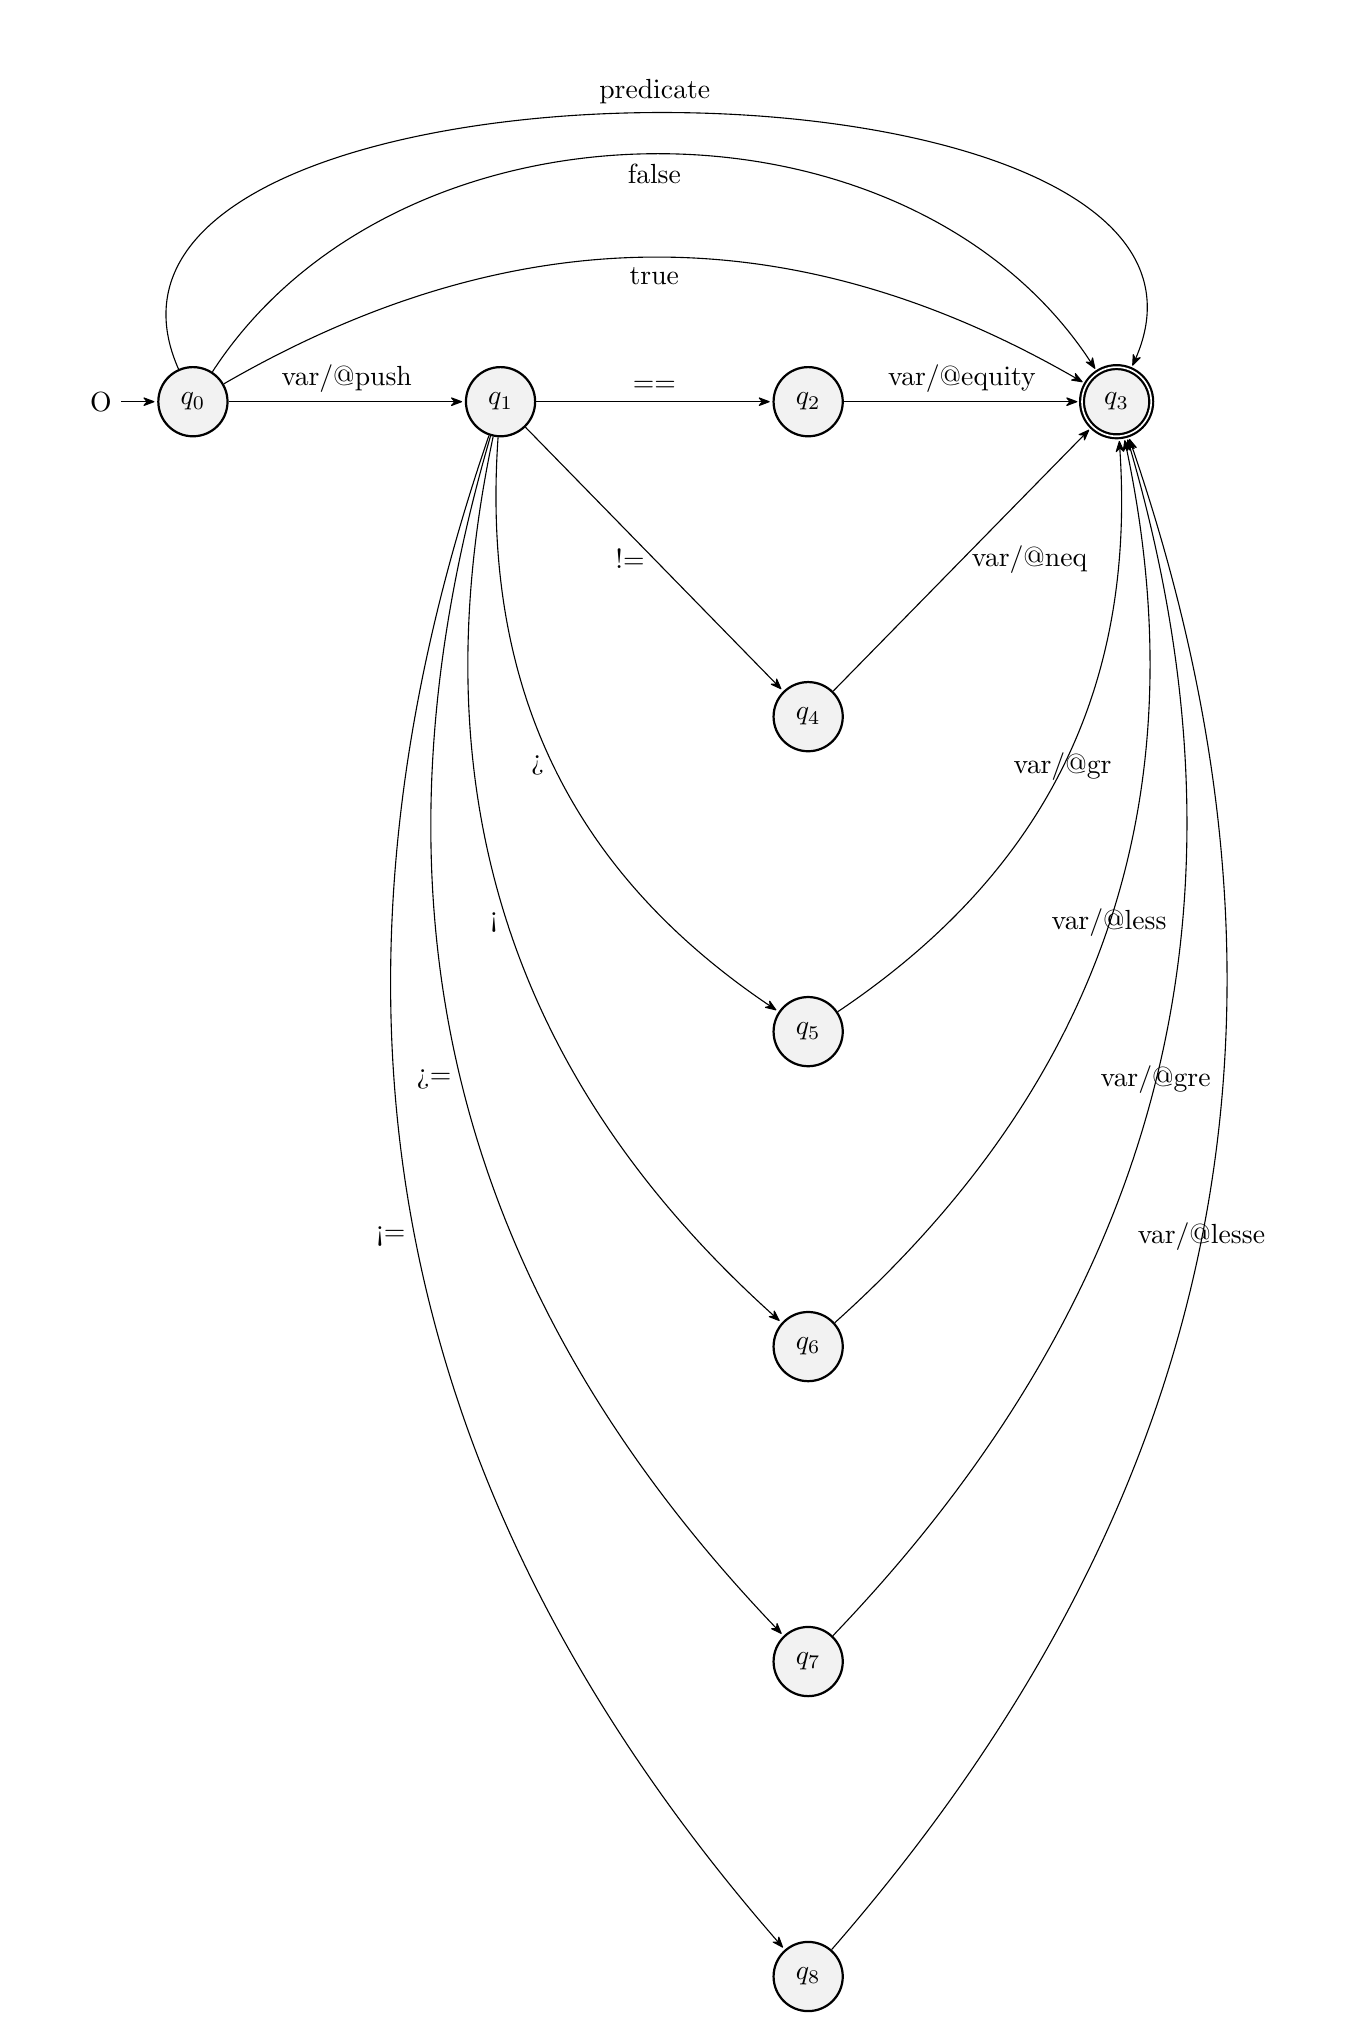
\begin{tikzpicture}[node distance=4cm]
        \node[state,initial, initial text=O] (q0) {$q_0$};
        \node[state,right=3cm of q0] (q1) {$q_1$};
        \node[state,right=3cm of q1] (q2) {$q_2$};
        \node[state,right=3cm of q2,accepting] (q3) {$q_3$};
        
        \draw (q0) edge[above] node{var/@push} (q1);
        \draw (q1) edge[above] node{==} (q2);
        \draw (q2) edge[above] node{var/@equity} (q3);

        \node[state,below of=q2] (q4) {$q_4$};
        \draw (q1) edge[left] node{!=} (q4);
        \draw (q4) edge[right] node{var/@neq} (q3);
        
        \node[state,below of=q4] (q5) {$q_5$};
        \draw (q1) edge[bend right] node[left]{>} (q5);
        \draw (q5) edge[bend right] node{var/@gr} (q3);
        
        \node[state,below of=q5] (q6) {$q_6$};
        \draw (q1) edge[bend right] node[left]{<} (q6);
        \draw (q6) edge[bend right] node{var/@less} (q3);
        
        \node[state,below of=q6] (q7) {$q_7$};
        \draw (q1) edge[bend right] node[left]{>=} (q7);
        \draw (q7) edge[bend right] node{var/@gre} (q3);
        
        \node[state,below of=q7] (q8) {$q_8$};
        \draw (q1) edge[bend right] node[left]{<=} (q8);
        \draw (q8) edge[bend right] node{var/@lesse} (q3);

        \draw (q0) edge[bend left] node[below]{true} (q3);
        \draw (q0) edge[bend left=2cm] node[below]{false} (q3);
        \draw (q0) edge[bend left=4cm] node[above]{predicate} (q3);

    \end{tikzpicture}

\end{latin}


%نام و نام خانوادگی:
%شماره دانشجویی: 
\مسئله{نام سؤال}

\پاسخ{}

\begin{latin}
    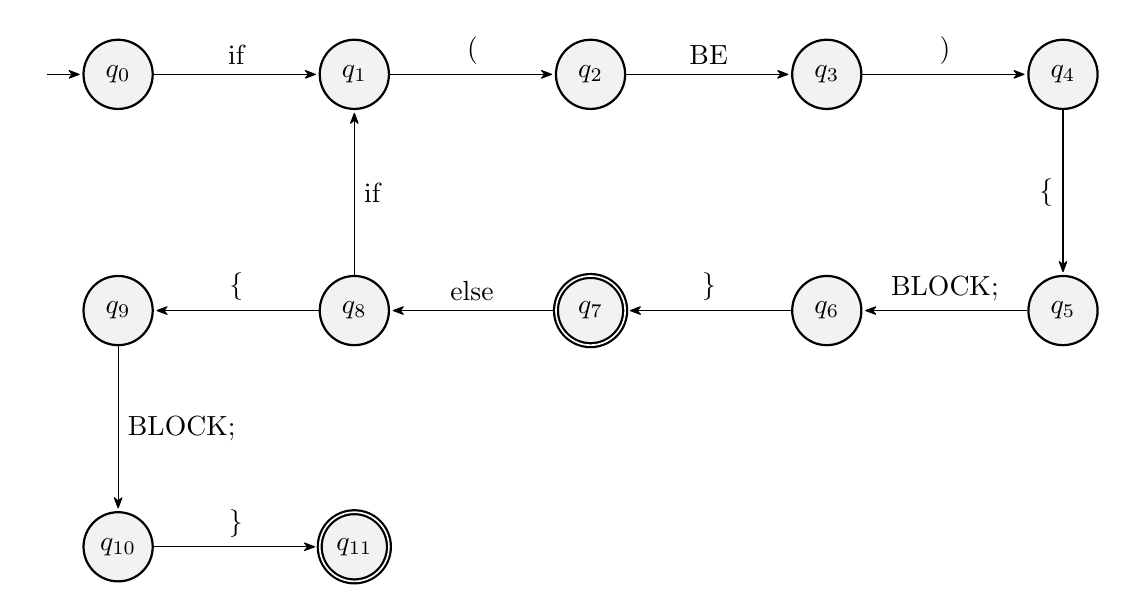
\begin{tikzpicture}
    
    \node[state,initial] (q0) {$q_0$};
    \node[state,right of=q0] (q1) {$q_1$};
    \node[state,right of=q1] (q2) {$q_2$};
    \node[state,right of=q2] (q3) {$q_3$};
    \node[state,right of=q3] (q4) {$q_4$};
    \node[state,below of=q4] (q5) {$q_5$};
    \node[state,left of=q5] (q6) {$q_6$};
    \node[state,left of=q6,accepting] (q7) {$q_7$};
    \node[state,left of=q7] (q8) {$q_8$};
    \node[state,left of=q8] (q9) {$q_9$};
    \node[state,below of=q9] (q10) {$q_{10}$};
    \node[state,right of=q10,accepting] (q11) {$q_{11}$};

    \draw (q0) edge[above] node{if} (q1);
    \draw (q1) edge[above] node{(} (q2);
    \draw (q2) edge[above] node{BE} (q3);
    \draw (q3) edge[above] node{)} (q4);
    \draw (q4) edge[left] node{\{} (q5);
    \draw (q5) edge[above] node{BLOCK;} (q6);
    \draw (q6) edge[above] node{\}} (q7);
    \draw (q7) edge[above] node{else} (q8);
    \draw (q8) edge[above] node{\{} (q9);
    \draw (q9) edge[right] node{BLOCK;} (q10);
    \draw (q10) edge[above] node{\}} (q11);
    \draw (q8) edge[right] node{if} (q1);

     \end{tikzpicture}
\end{latin}


%نام و نام خانوادگی:
%شماره دانشجویی: 
\مسئله{نام سؤال}

\پاسخ{}

الف) دیگر بین ضرب و جمع الویتی قائل نیستیم و هر کدام که زودتر بیاید آن را انجام می‌دهیم.
به این صورت که ابتدا ۴ را با ۳ جمع کرده و حاصل ۷ را حساب می‌کنیم و سپس این حاصل را در ۶ ضرب می‌کنیم و جواب می‌شود ۴۲. در حالی که همه میدانیم که ابتدا باید ۳ در ۶ ضرب شود که بشود ۱۸ و بعد با ۴ جمع بشود که بشود ۲۲.

ب) 

\begin{latin}
    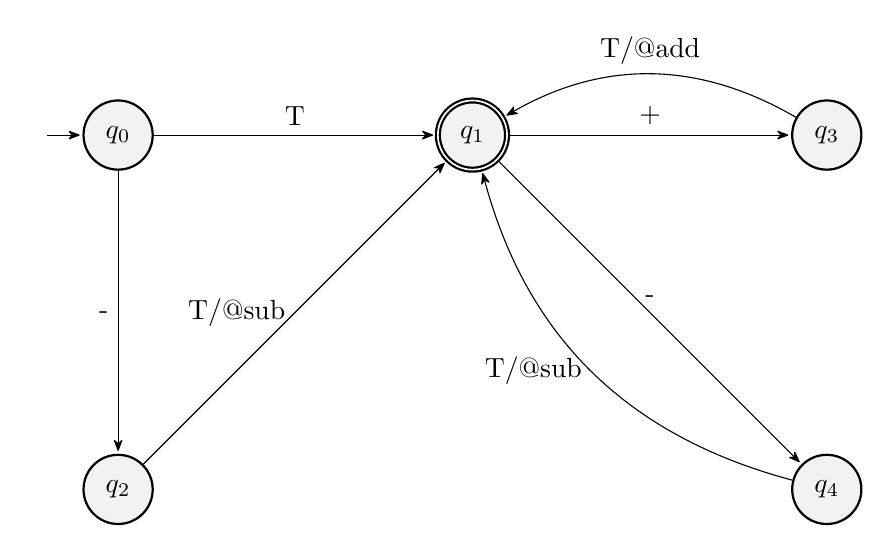
\begin{tikzpicture}[node distance=4.5cm]
        \node[state, initial] (q0) {$q_0$};
        \node[state, right of=q0,accepting] (q1) {$q_1$};
        \node[state, below of=q0] (q2) {$q_2$};
        \node[state, right of=q1] (q3) {$q_3$};
        \node[state, below of=q3] (q4) {$q_4$};
        
        \draw (q0) edge[above] node{T} (q1);
        \draw (q0) edge[left] node{-} (q2);
        \draw (q2) edge[left] node{T/@sub} (q1);
        \draw (q1) edge[above] node{+} (q3);
        \draw (q1) edge[above] node{-} (q4);
        \draw (q4) edge[bend left] node[left]{T/@sub} (q1);
        \draw (q3) edge[bend right] node[above]{T/@add} (q1);
        
    \end{tikzpicture}

    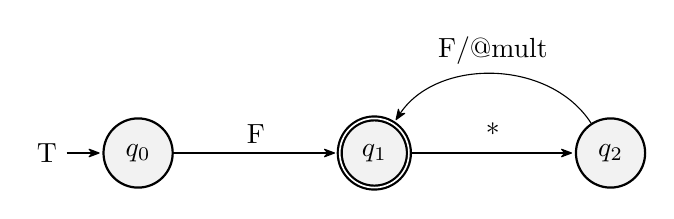
\begin{tikzpicture}
        \node[state,initial,initial text=T] (q0) {$q_0$};
        \node[state,accepting,right of=q0] (q1) {$q_1$};
        \node[state,right of=q1] (q2) {$q_2$};

        \draw (q0) edge[above] node{F} (q1);
        \draw (q1) edge[above] node{*} (q2);
        \draw (q2) edge[bend right=2cm] node[above]{F/@mult} (q1);
    \end{tikzpicture}

    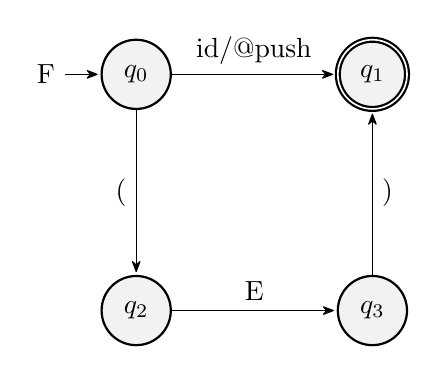
\begin{tikzpicture}
        \node[state,initial,initial text=F] (q0) {$q_0$};
        \node[state,right of=q0,accepting] (q1) {$q_1$};
        \node[state,below of=q0] (q2) {$q_2$};
        \node[state,below of=q1] (q3) {$q_3$};
    
        \draw (q0) edge[above] node{id/@push} (q1);
        \draw (q0) edge[left] node{$($} (q2); 
        \draw (q2) edge[above] node{E} (q3);
        \draw (q3) edge[right] node{$)$} (q1);
    \end{tikzpicture}

\end{latin}


%نام و نام خانوادگی:
%شماره دانشجویی: 
\مسئله{نام سؤال}

\پاسخ{}

\begin{latin}
\begin{center}
    $\color{red}id\color{black}*(id+id)$
    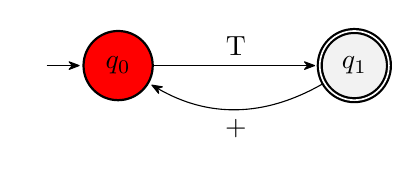
\begin{tikzpicture}
    
        \node[state,initial,fill=red] (q0) {$q_0$};
        \node[state,right of=q0,accepting] (q1) {$q_1$};
    
        \draw (q0) edge[above] node{T} (q1);
        \draw (q1) edge[bend left] node[below]{+} (q0);
    
    \end{tikzpicture}
    \begin{tabular}{ | l |  l | }
        \hline
        $q_1$ & T\_constInt \\ \hline
        $q_2$ & + \\ \hline
        $q_3$ & - \\ \hline
        $q_4$ & * \\ \hline
        $q_5$ & / \\ \hline
        $q_8$ & T\_comment \\ 
        \hline
    
    \end{tabular}
\end{center}
\end{latin}
   
\end{document}

